
\subsection{JSBMLInterface package}

In questa sezione descriveremo il package \textbf{JSBMLInterface}.

Questo package contiene le implementazioni dei concetti che riguardano
l'interfacciamento con il modello SBML e in particolare con la
libreria JSBML (vedi \cite{JSbmlDistribution}). 

\subsubsection*{Supplied Abstractions}

Le astrazioni fornite da questo package sono le seguenti:
\begin{itemize}
\item astrarre dalla libreria JSBML e dal suo modello dati. In questo
  modo l'unico contesto del progetto dipendente dalla libreria JSBML
  \`e confinato a questo singolo package. Questo permette agli altri
  package di non essere a conoscenza della specifica "sorgente" che
  fornisce il modello, in quanto se si vorr\`a sostituire libreria di
  interfacciamento con modelli SBML, sar\`a necessario apportare le
  modifiche solo in questo package, lasciando tutto il restante codice
  del progetto inalterato.
\item interpretare il modello fornito dalla libreria JSBML, costruire
  gli elementi fondamentali del nostro modello dati e renderlo
  disponibile per iniziare successive computazioni.
\end{itemize}

\subsubsection*{Class diagram}

Riporto una versione semplificata del diagramma delle classi di questo
pacchetto, disegnando solo quelle classi di interesse per la
trattazione.
\begin{figure}
  \centering
  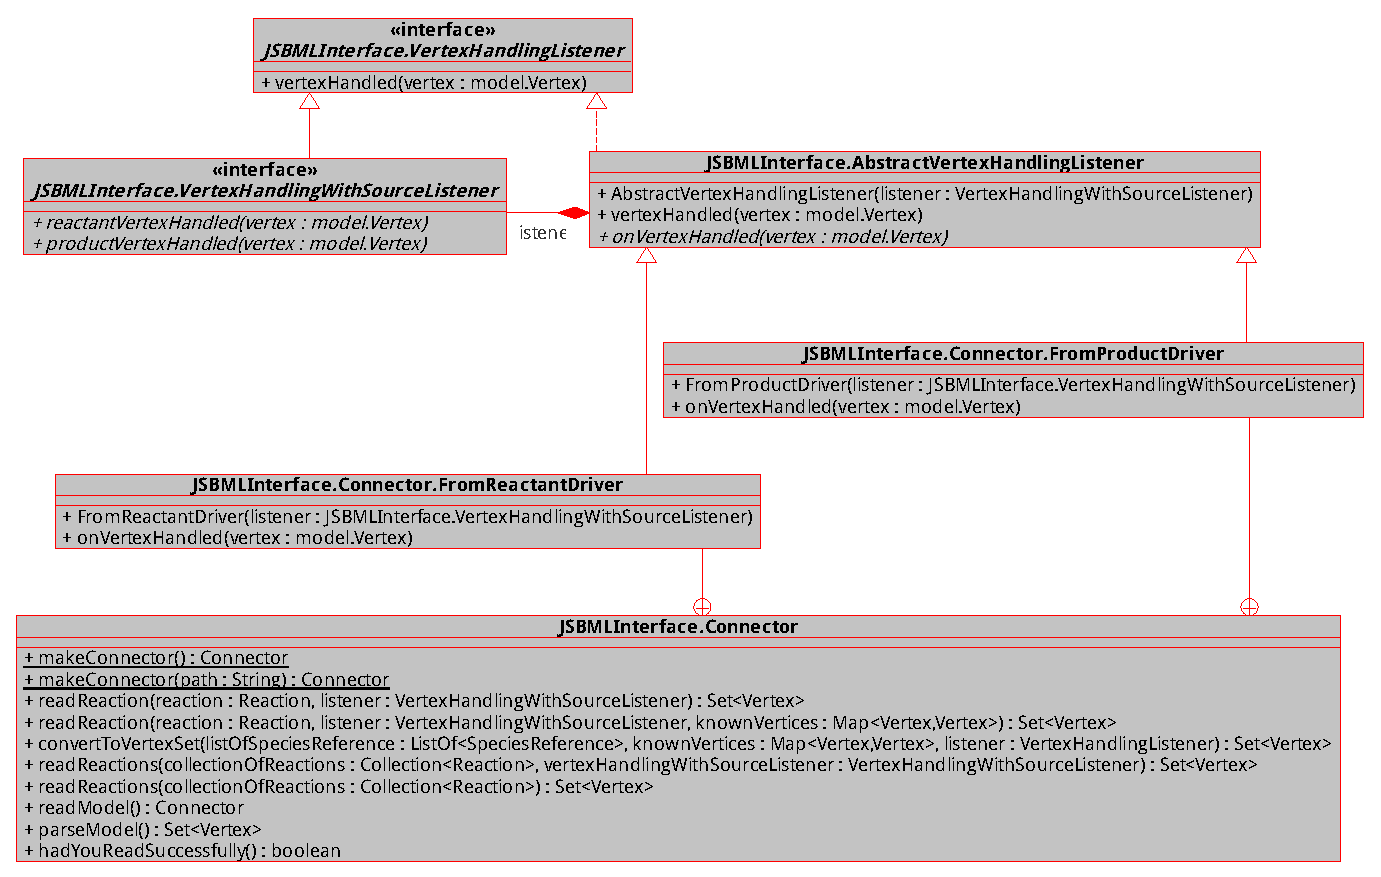
\includegraphics[angle=90]{packages/JSBMLInterface-class-diagram.eps}
  \caption{JBSMLInterface package's classes}
  \label{fig:JSBMLInterface-ClassDiagram}
\end{figure}

In questo package la classe principale e che merita qualche
spiegazione \`e \emph{Connector}.

Questa classe incapsula la responsabilit\`a di delegare alla libreria
JSBML la lettura di un modello SBML e successivamente interpretare il
risultato di tale lettura in modo da costruire un nostro modello dati
interno, input di successive computazioni.

La parte di interpretazione del modello letto dalla libreria JSBML \`e
quella pi\`u interessante, in quanto permette di elaborare e
selezionare solo quelle informazioni del modello SBML che
effettivamente sono necessarie al nostro lavoro, come descritto nella
sezione "\nameref{sec:necessaryRealObjectsModeledInSBML}". 

Questo procedimento \`e implementato principalmente nel metodo
\emph{readReactions}, il quale permette di costruire un insieme di
vertici che verranno usati per costruire il nostro modello di dominio,
a partire da una collezione di reazioni, risultato della lettura della
libreria SBML. Inoltre, come spiegher\`o nella prossima sezione, \`e
possibile passare come argomento un \emph{listener} da notificare ogni
qualvolta si costruisce un nuovo vertice per il modello da costruire.

Quello che viene fatto \`e di scandire ogni reazione e, per ognuna, si
creano tanti vertici tanti sono gli oggetti appartenenti agli insiemi
\emph{reactants} e \emph{products}, prestando attenzione a non
costruire nuovi vertici per species gi\`a analizzate.